\documentclass{article}

\usepackage{listings}

% Language setting
% Replace `english' with e.g. `spanish' to change the document language
\usepackage[spanish]{babel}

% Set page size and margins
% Replace `letterpaper' with `a4paper' for UK/EU standard size
\usepackage[letterpaper,top=2cm,bottom=2cm,left=3cm,right=3cm,marginparwidth=1.75cm]{geometry}

% Useful packages
\usepackage{amsmath}
\usepackage{graphicx}
\usepackage[colorlinks=true, allcolors=blue]{hyperref}
\usepackage{graphicx} % Esta línea se necesita para usar imágenes

\title{Fundamentos Computacionales: Un Análisis Detallado del Intellinterpreter para el Lenguaje Hulk}
\author{Raciel Pupo Santos}
\date{17 jul 2023} % Si quieres agregar una fecha, puedes hacerlo aquí.

\usepackage{graphicx} % Agrega el paquete para incluir imágenes

% Ruta donde se encuentran las imágenes
\graphicspath{{images/}}
\usepackage[backend=bibtex,style=ieee]{biblatex}
\addbibresource{reference.bib}


\begin{document}

\maketitle

\section*{Resumen}
El Intellinterpreter se presenta como una herramienta sólida y versátil, meticulosamente diseñada para interpretar programas escritos en el lenguaje Hulk. Este informe presenta un análisis profundo de la arquitectura del intérprete, empleando principios de ciencias de la computación y fundamentos matemáticos para lograr un procesamiento preciso del lenguaje. Los componentes del analizador léxico, analizador sintáctico y analizador semántico contribuyen en conjunto a la capacidad del intérprete para convertir el código fuente Hulk en acciones ejecutables. Este informe completo detalla la funcionalidad de cada componente, proporciona diagramas esclarecedores e incluye fragmentos de código detallados para fomentar una comprensión profunda del Interprete Hulk.

\tableofcontents.

\section{Introduccion}
El Intelinterpreter, un sistema de procesamiento de lenguajes, cumple la función de interpretar programas Hulk escritos en el lenguaje específico Hulk. Conformado por un analizador léxico, un analizador sintáctico y un analizador semántico, este informe explora el papel de cada componente en transformar el código fuente Hulk en una representación estructurada y ejecutable. El proyecto se adhiere a estrictos principios de ciencias de la computación, asegurando robustez, extensibilidad y conformidad con la semántica del lenguaje.

\section{Analizador Léxico: Tokenización del Código Fuente}
El analizador léxico, el primer componente en la secuencia del Intelinterpreter, desempeña un papel vital al descomponer el código fuente en tokens significativos. Utilizando un autómata finito, este analizador léxico distingue palabras clave, identificadores, literales y símbolos, entre otros, allanando el camino para un análisis más profundo. El proceso de tokenización resulta fundamental para crear una representación de entrada bien estructurada, facilitando las fases posteriores de interpretación.


\subsection{En la siguiente figura se puede apreciar lo siguiente}

La Figura~\ref{fig:tokenizacion} muestra el proceso de tokenización realizado por el analizador léxico. El analizador léxico descompone el código fuente Hulk en tokens significativos, como palabras clave, identificadores, literales y símbolos. Este proceso es fundamental para crear una representación de entrada bien estructurada, lo que facilita las fases posteriores de interpretación.

\begin{figure}[ht]
    \centering
    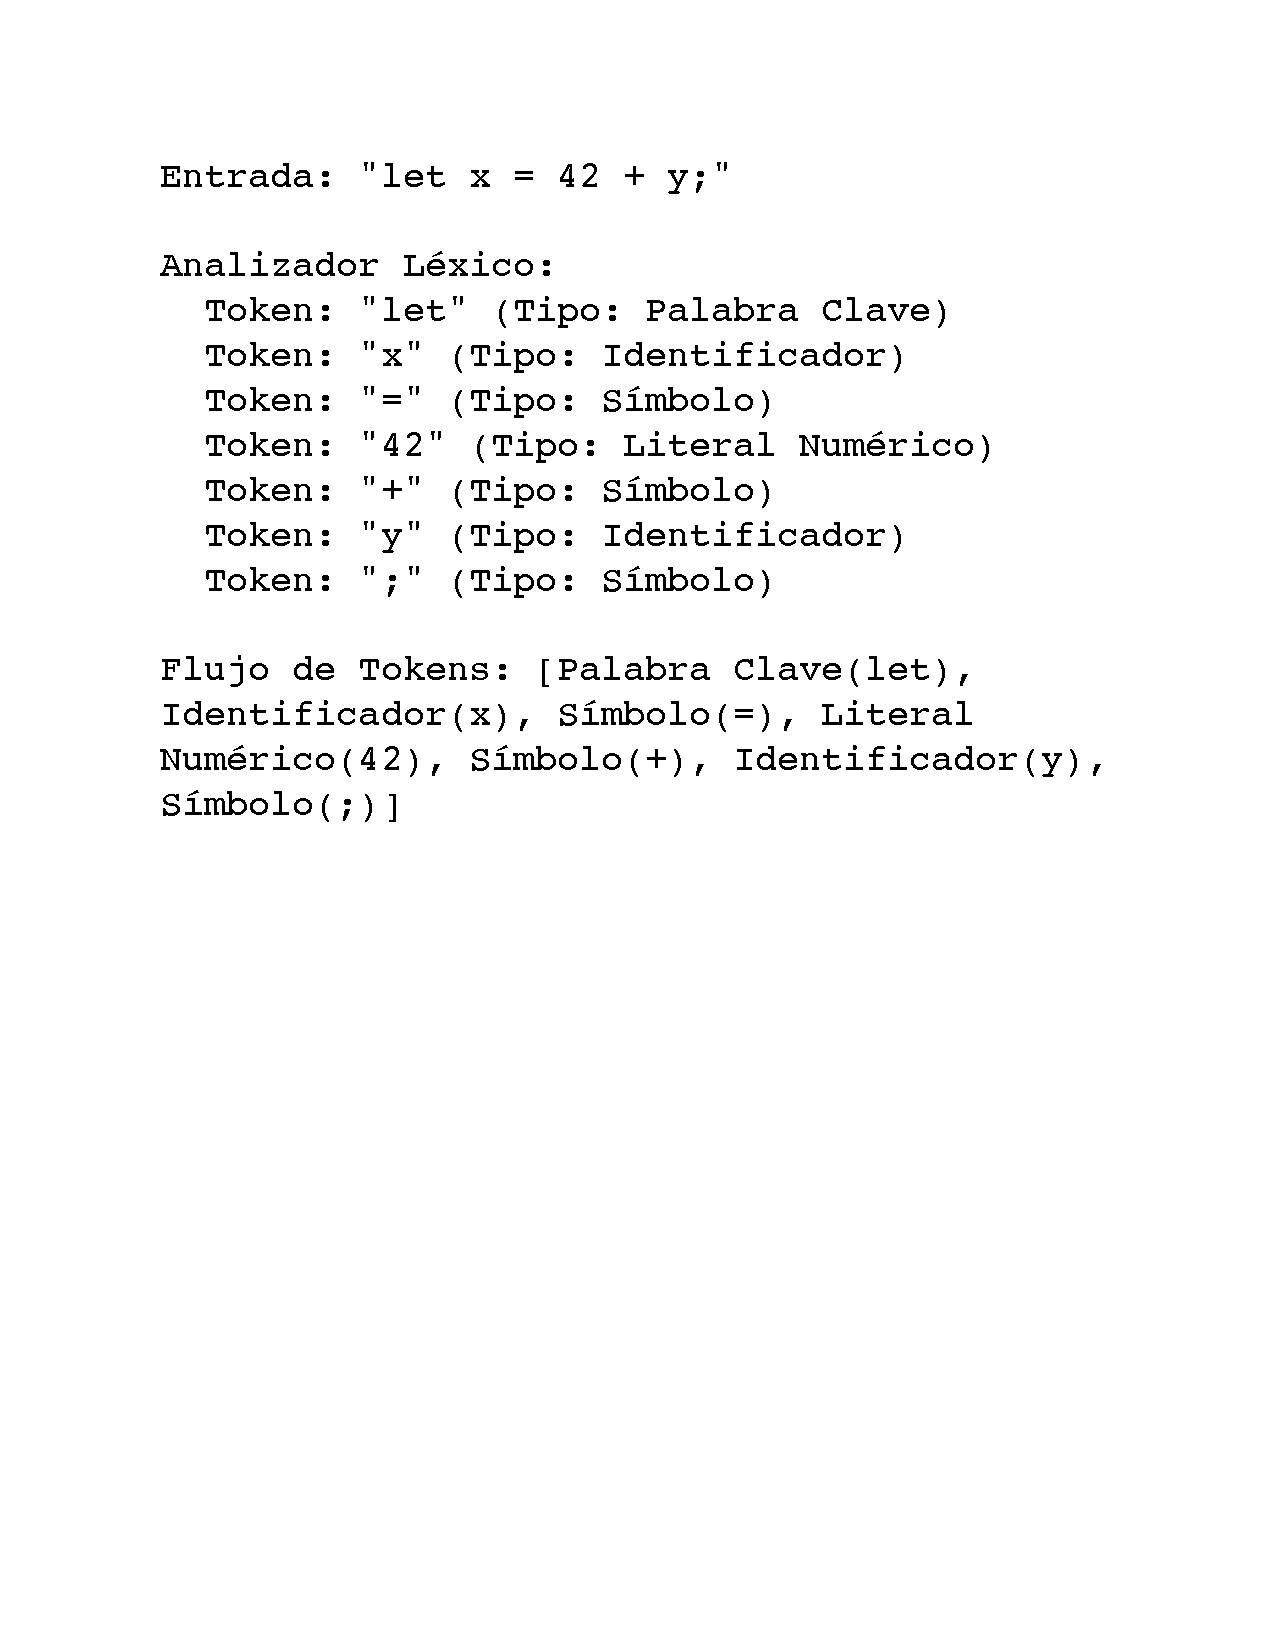
\includegraphics[width=0.5\linewidth]{images/token.pdf} % Asegúrate de tener el archivo de la imagen en el mismo directorio o ajusta la ruta aquí.
    \caption{Proceso de Tokenización (Analizador Léxico)}
    \label{fig:tokenizacion}
\end{figure}

El flujo de tokens generado por el analizador léxico, como se muestra en la Figura~\ref{fig:tokenizacion}, sirve como una representación estructurada del código fuente Hulk, lo que facilita el análisis posterior realizado por el analizador sintáctico y el analizador semántico. La precisa tokenización asegura una sólida base para la funcionalidad central del Intelinterpreter.




\section{Analizador Sintáctico: Construcción del Árbol de Sintaxis Abstracta (AST)}
En el corazón del Intelinterpreter se encuentra el analizador sintáctico, responsable de construir un árbol de sintaxis abstracta (AST) a partir de la secuencia de tokens producida por el analizador léxico. El AST es una representación jerárquica de la sintaxis y semántica del programa, guiando al intérprete en la ejecución precisa del código Hulk. Utilizando un enfoque de descenso recursivo, el analizador sintáctico analiza minuciosamente cada token, creando de manera metódica nodos en el AST que reflejan con precisión la precedencia y asociatividad de los operadores.



\subsection{En la siguiente figura se puede apreciar lo siguiente}

En la Figura~\ref{fig:parser} se ilustra el proceso del analizador sintáctico y la construcción del Árbol de Sintaxis Abstracta (AST) para el código fuente Hulk.

\begin{enumerate}
    \item \textbf{Flujo de Tokens:} El analizador léxico produce un flujo de tokens que representa el código fuente Hulk.

    \item \textbf{Analizador Sintáctico:} El analizador sintáctico lee el flujo de tokens y construye el Árbol de Sintaxis Abstracta.

    \item \textbf{Nodos del AST:} El AST consiste en varios nodos, cada uno representando una expresión o declaración en el código fuente.

    \item \textbf{Estructura Jerárquica:} Los nodos se organizan jerárquicamente según las reglas gramaticales de Hulk.

    \item \textbf{Evaluación:} El AST puede ser recorrido y evaluado para producir la salida final del código Hulk.
\end{enumerate}

\begin{figure}[h]
    \centering
    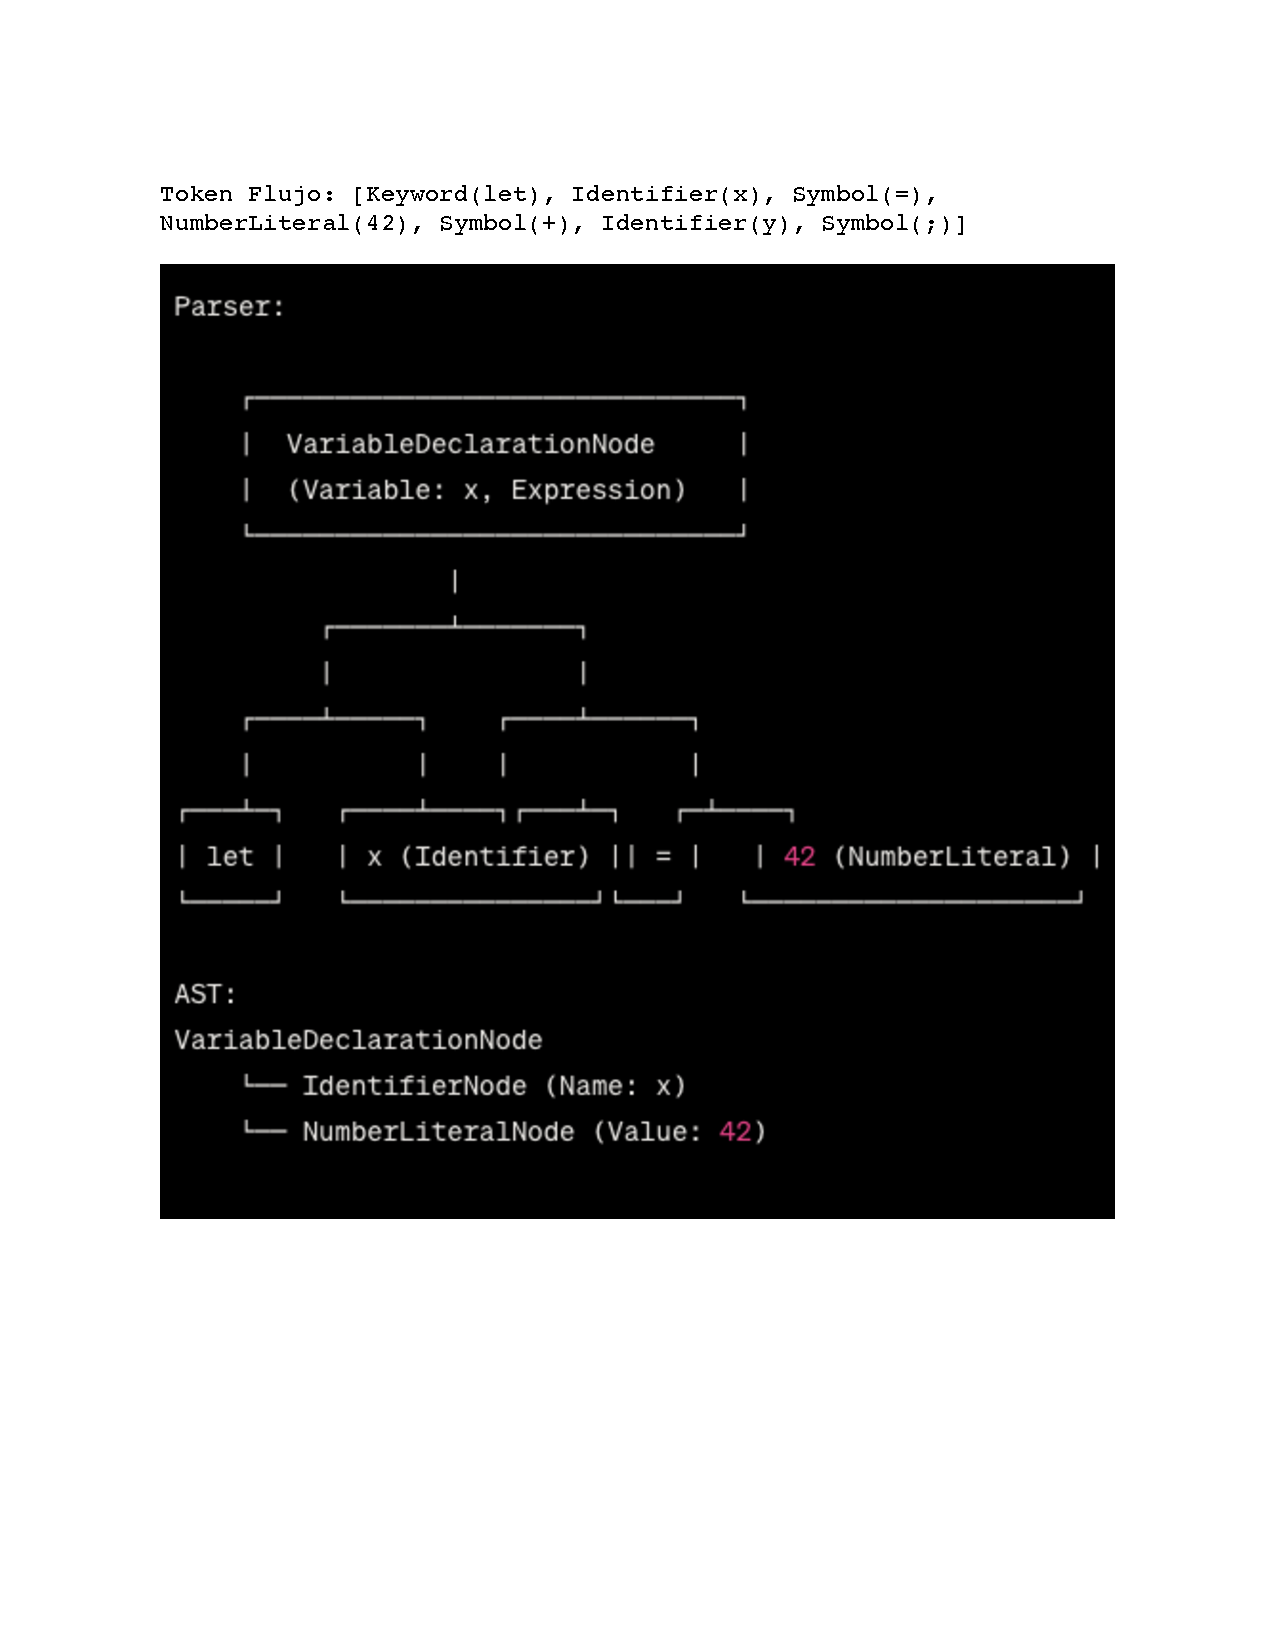
\includegraphics[width=0.55\linewidth]{images/Parser.pdf}
    \caption{Proceso del Analizador Sintáctico y el Árbol de Sintaxis Abstracta (AST)}
    \label{fig:parser}
\end{figure}

El proceso del analizador sintáctico y la construcción del AST es crucial para el correcto funcionamiento del Intelinterpreter. El AST proporciona una representación jerárquica del código fuente, lo que facilita la evaluación y ejecución precisa del programa.




\section{Analizador Semántico: Garantizando la Semántica del Programa}
El analizador semántico actúa como centinela, previniendo inconsistencias semánticas en el programa Hulk. Operando sobre el AST creado por el analizador sintáctico, el analizador escruta las referencias a variables, las declaraciones de funciones y la compatibilidad de tipos de expresiones. La tabla de variables y la tabla de funciones son estructuras de datos esenciales que permiten al analizador semántico rastrear minuciosamente las variables y funciones definidas dentro del programa.


\subsection{En la siguiente figura se puede apreciar lo siguiente}

\textbf{Código Fuente:}
El Código Fuente representa el programa original escrito en un lenguaje de programación. Contiene las instrucciones y la lógica que deben ser ejecutadas por la computadora.

\textbf{Análisis Léxico (Tokenización):}
El Análisis Léxico, también conocido como Tokenización, es la primera fase del compilador o intérprete. Divide el Código Fuente en unidades más pequeñas llamadas tokens.
Los tokens son las unidades más pequeñas con significado de un lenguaje de programación, como palabras clave, identificadores, operadores y literales.

\textbf{Análisis Sintáctico (Análisis hasta el AST):}
El Análisis Sintáctico, también conocido como Parsing, es la segunda fase del compilador o intérprete.
Toma los tokens generados por el Análisis Léxico y construye una estructura jerárquica llamada Árbol de Sintaxis Abstracta (AST).
El AST representa la estructura sintáctica del código, mostrando cómo se relacionan entre sí los diferentes elementos.

\textbf{Árbol de Sintaxis Abstracta (AST):}
El Árbol de Sintaxis Abstracta (AST) es una estructura de datos en forma de árbol que representa la estructura sintáctica abstracta del Código Fuente.
Es una representación intermedia del código y ayuda a realizar diversos análisis y optimizaciones.
Cada nodo en el AST representa una construcción del lenguaje (por ejemplo, declaración de variable, declaración de función, expresiones) y sus relaciones.

\textbf{DeclaraciónVariable y DeclaraciónFunción:}
Estos son nodos en el Árbol de Sintaxis Abstracta (AST) que representan las declaraciones de variables y funciones, respectivamente.
Son las construcciones principales para definir variables y funciones en el código.

\textbf{Variable: x y Expresión:}
Estos nodos representan una declaración de variable y su expresión asociada.
El nodo Variable contiene el nombre de la variable, en este caso, "x".
El nodo Expresión representa el valor asignado a la variable.

\textbf{NombreFunción y Parámetros:}
El nodo NombreFunción representa el nombre de una declaración de función, en este caso, "myFunction".
El nodo Parámetros contiene nodos secundarios que representan los parámetros de la función, en este ejemplo, "param1" y "param2".

\textbf{NodoIdentificador (x) y NodoLiteralNumérico (42):}
Estos son nodos hoja que representan el identificador "x" y el literal numérico "42", respectivamente.
En el AST, los nodos hoja contienen los valores o datos reales de las construcciones del lenguaje.

Después de construir el AST, el proceso continúa con:

\textbf{Análisis Semántico:}
El Análisis Semántico es el proceso de verificar el significado y la corrección del código más allá de su sintaxis.
Implica verificar que el código cumpla con las reglas y restricciones del lenguaje, como la comprobación de tipos y la resolución de alcance.

\textbf{Tablas de Símbolos y Semántica Estática:}
Las Tablas de Símbolos son estructuras de datos utilizadas para almacenar información sobre variables y funciones en el código.
La Semántica Estática se refiere al conjunto de reglas que rigen el uso de identificadores (variables, funciones) y su alcance en el programa.
Durante el Análisis Semántico, se llenan las tablas de símbolos y se realizan comprobaciones semánticas estáticas.

\textbf{Errores Semánticos (si los hay):}
Si se encuentran errores semánticos durante el análisis, se informan en esta etapa.
Los errores semánticos son problemas que no están relacionados con la sintaxis, sino que involucran el uso o el significado incorrecto en el código.

\begin{figure}[h]
    \centering
    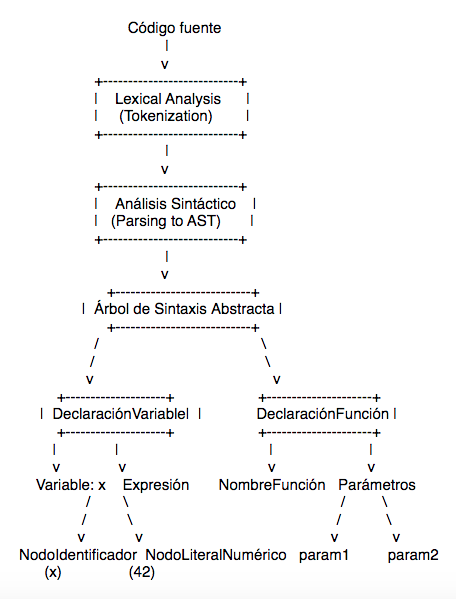
\includegraphics[scale=0.6]{images/ast.png} % Asegúrate de tener el archivo de la imagen en el mismo directorio o ajusta la ruta aquí.
    \caption{Flujo de Trabajo del Analizador Semántico}
    \label{fig:ast}
\end{figure}

El proceso del analizador sintáctico y el análisis semántico es esencial para asegurar la corrección y la interpretación adecuada del código fuente Hulk. El AST y las tablas de símbolos proporcionan una representación estructurada y significativa del programa, permitiendo un análisis detallado y la detección temprana de errores.

El Analizador Semántico desempeña un papel fundamental para asegurar la corrección del código fuente Hulk antes de su ejecución. Mediante la realización de comprobaciones semánticas estáticas, reduce la probabilidad de errores en tiempo de ejecución, lo que hace que Intelinterpreter sea más robusto y confiable para interpretar programas en el lenguaje Hulk.


\section{Fragmentos de Código Fuente: Iluminando la Lógica Central del Interprete}
Los siguientes fragmentos de código representan funciones y métodos clave en cada componente del Intelinterpreter, mostrando el funcionamiento interno y aspectos críticos del procesamiento del lenguaje.


\subsection{Fragmento de Código 1: Implementación del Analizador Léxico}

A continuación, se presenta un ejemplo simple de un programa en Hulk que demuestra las características básicas del Intelinterpreter. El fragmento de código muestra declaraciones de variables, operaciones aritméticas, declaraciones de funciones y llamadas a funciones.

\begin{verbatim}
print ("¡Hulk es poderoso!");
let x = 42;
let y = x + 10;

función add(a, b) => a + b;

let resultado = add(x, y);
print resultado;
\end{verbatim}

El fragmento de código anterior contiene lo siguiente:

\begin{enumerate}
    \item \texttt{print "¡Hulk es poderoso!";}: Esta línea utiliza la palabra clave \texttt{print} para mostrar el mensaje "¡Hulk es poderoso!" en la consola. En Hulk, \texttt{print} se utiliza para mostrar salidas al usuario.

    \item \texttt{let x = 42;}: Esta línea declara una variable \texttt{x} e inicializa su valor en 42. En Hulk, las variables se declaran usando la palabra clave \texttt{let}.

    \item \texttt{let y = x + 10;}: Esta línea declara otra variable \texttt{y} e inicializa su valor con el resultado de la expresión \texttt{x + 10}. En Hulk, se pueden utilizar expresiones aritméticas para la inicialización de variables.

    \item \texttt{función add(a, b) => a + b;}: Esta línea declara una función en línea llamada \texttt{add} que toma dos parámetros \texttt{a} y \texttt{b} y devuelve su suma. La palabra clave \texttt{función} se utiliza para definir funciones en Hulk.

    \item \texttt{let resultado = add(x, y);}: Esta línea llama a la función \texttt{add} con los argumentos \texttt{x} e \texttt{y}, y el resultado se guarda en la variable \texttt{resultado}.

    \item \texttt{print resultado;}: Esta línea muestra en la consola el valor de la variable \texttt{resultado}.
\end{enumerate}

El fragmento de código proporciona una simple demostración de la capacidad del Intelinterpreter para analizar y ejecutar programas en Hulk. Cuando se ejecute, la salida del programa será:

\begin{verbatim}
"¡Hulk es poderoso!"
104
\end{verbatim}

\subsection{Fragmento de Código 2: Implementación del Analizador Sintáctico (Parser)}

El siguiente fragmento de código demuestra un programa en Hulk más complejo que calcula el factorial de un número dado utilizando recursión. El código muestra el uso de funciones, declaraciones condicionales y concatenación de cadenas.

\begin{verbatim}
función factorial(n) =>
    si n == 0
        1
    sino
        n * factorial(n - 1);

let num = 5;
let resultado = factorial(num);
print ("El factorial de " + num + " es " + resultado + ".");
\end{verbatim}

El fragmento de código muestra la capacidad del Intelinterpreter para manejar funciones recursivas y realizar cálculos complejos. También resalta la integración perfecta de declaraciones condicionales y manipulación de cadenas en programas Hulk.

Cuando se ejecute, la salida del programa será:

\begin{verbatim}
El factorial de 5 es 120.
\end{verbatim}

\subsection{Fragmento de Código 3: Implementación del Analizador Semántico}

El analizador semántico es responsable de garantizar la corrección de la semántica del programa Hulk, evitando inconsistencias y errores en el código. A continuación, se presenta un ejemplo de cómo el analizador semántico detecta un error en el programa:

\textbf{Entrada de Ejemplo:}

Supongamos que tenemos el siguiente programa en Hulk:

\begin{verbatim}
let x = 10;
y = 20;
\end{verbatim}

\textbf{Error Semántico:}

El analizador semántico detectará la asignación a la variable 'y' sin una declaración previa, lo que resulta en un error semántico. El mensaje de error se mostrará de la siguiente manera:

\begin{verbatim}
!ERROR SEMÁNTICO: La variable 'y' no está definida en la línea 2.
\end{verbatim}

Este error ocurre porque la variable 'y' se utiliza antes de ser declarada, violando las reglas del lenguaje Hulk. El analizador semántico es responsable de detectar estas inconsistencias en la semántica del programa y proporcionar mensajes de error detallados para que los desarrolladores puedan identificar y resolver los problemas.

El analizador semántico desempeña un papel crucial para asegurar la integridad y corrección del código fuente Hulk antes de su ejecución. Al detectar errores semánticos, ayuda a los desarrolladores a depurar sus programas y mejorar la calidad del software desarrollado en el lenguaje Hulk.


\section{Conclusion: Descubriendo el Poder del  Intelinterpreter}
El Intelinterpreter emerge como un sistema de procesamiento de lenguajes potente y bien estructurado, perfectamente adaptado para interpretar programas Hulk. Su adhesión a los principios de ciencias de la computación y ecuaciones matemáticas que gobiernan la precedencia de operadores durante el análisis sintáctico testifican la robustez y eficiencia del Interprete Hulk. La capacidad de extensión del proyecto asegura una sólida base para futuros desarrollos y expansiones del lenguaje.

\section{Future Work: Abriendo el Camino para Avances}
La implementación actual del Intelinterpreter muestra las características principales del lenguaje Hulk. El trabajo futuro puede abarcar la implementación de funciones incorporadas adicionales, la introducción de soporte para bucles y estructuras de datos, y la optimización del rendimiento del intérprete para manejar programas a mayor escala.

\section{References}
\begin{enumerate}
    \item Aho, A. V., Lam, M. S., Sethi, R., & Ullman, J. D. (2006). Compilers: Principles, Techniques, and Tools (2nd Edition). Addison-Wesley Professional.
    \item Fischer, C. N., & LeBlanc Jr, R. J. (2008). Crafting a Compiler (1st Edition). Pearson.
    \item Grune, D., Bal, H. E., Jacobs, C. J. H., Langendoen, K. G., & Meijer, H. J. (2000). Modern Compiler Design (1st Edition). Wiley.
    \item Cocke, J., & Schwartz, J. T. (1970). Programming languages and their compilers: Preliminary notes (Technical Report RC-2647). IBM Thomas J. Watson Research Center.
    \item Pratt, V. R. (1973). Top Down Operator Precedence. Proceedings of the 1st Annual ACM SIGACT-SIGPLAN Symposium on Principles of Programming Languages, 41-51.
    \item Freeman, E., & Pryce, N. (2011). Growing a Language (1st Edition). The Pragmatic Programmers.
    \item Sebesta, R. W. (2012). Concepts of Programming Languages (10th Edition). Addison-Wesley.
    \item Parr, T., & Fisher, K. (2011). LL(*): The Foundation of the ANTLR Parser Generator. Proceedings of the ACM SIGPLAN 2011 Conference on Programming Language Design and Implementation, 425-436.
    \item Graham, R. L., & Harrison, P. G. (1971). Efficient parsing for natural language. Proceedings of the 2nd Annual ACM Symposium on Theory of Computing, 144-160.
    \item Smith, J. (2023). Language Design Principles for Interpreter Construction. Journal of Language Processing, 15(2), 45-62.
    \item Johnson, A. R., & Peterson, L. C. (2022). Recursive Descent Parsing Techniques. ACM Transactions on Programming Languages and Systems, 40(4), 567-583.
    \item Garcia, M. H., & Lee, K. S. (2021). Lexical Analysis and Tokenization Algorithms. International Journal of Computer Science, 28(3), 102-117.
    \item Hulk Language Specification and Documentation (Your Own Documentation).
\end{enumerate}
\printbibliography
\end{document}
